\chapter{Cinematica del punto materiale} %1
%-------------------------------------------------------------------------------------------
\begin{figure}[htbp]
    \begin{center}
        \includegraphics[width=10cm]{images/assi.png} 
        \caption{Sistema di riferimento cartesiano: punto materiale $(P)$,
        raggio vettore $\vec r$.}
    \end{center}
\end{figure}

\section{Moto rettilineo uniforme}
%---------------------------------------------------------------------------
Un moto rettilineo uniforme è un moto che avviene lungo una retta
a velocità costante,
dunque può sempre essere ricondotto ad un moto unidimensionale.\\
Supponiamo di avere dunque un punto materiale nello spazio,
che si muove di velocità generica costante $v_0$.\\
Ricaviamo le equazioni del moto:
\begin{equation}
    \vec v_{(t)} = \vec v_0 = cost\quad\quad\quad
    \vec v_{(t)} = \frac{d\vec x}{dt}
\label{eq:velocity}
\end{equation}
Integrando tra l'istante iniziale e quello finale otterremo la
legge oraria di un moto rettilineo uniforme:
\begin{equation}
    \vec x_{(t)} = \vec x_0 + \int_{t_0}^{t}dt' \vec v_{(t')}\seg
    \boxed{\vec x_{(t)} = \vec x_0 +\vec v_0\sx t - t_0\dx}
\label{eq:MRU}
\end{equation}
Dove $t_0$ ed $\vec x_0$ sono rispettivamente, istante e
posizione iniziali.
\section{Moto rettilineo uniformemente accelerato}
%---------------------------------------------------------------------------
In questo caso è l'accelerazione ad essere costante nel tempo
ne segue che:
\begin{equation}
    \vec a_{(t)} = \vec a_0 \quad\quad\quad \vec a_{(t)} = \frac{d\vec v}{dt} = 
    \frac{d^2\vec x}{dt^2}
\label{eq:acceleration}
\end{equation}
Per ricavare la legge oraria del moto uniformemente accelerato,
dobbiamo integrare due volte nel tempo, dato che l'accelerazione
è la derivata seconda del vettore $\vec x$.
\begin{multline}
    \vec v_{(t)} = \vec v_0 + \int_{t_0}^{t}dt' \vec a_{(t')} =  \vec v_0 +  \vec a_0\sx t - t_0\dx\seg
    \\\seg\boxed{\vec x_{(t)} = \vec x_0 +\vec v_0\sx t - t_0\dx + \frac12\vec a_0\sx t-t_0\dx^2}
\label{eq:MRUA}
\end{multline}

\subsection{Relazione tra velocità ed accelerazione in funzione dello spazio}
Ora vedremo un modo per legare le grandezze velocità ed 
accelerazione, considerando la loro dipendenza dalla posizione
invece che dal tempo.\\
In questo esempio però ci mettiamo nel sistema di riferimento 
in cui il moto si svolge lungo una retta, che chiameremo asse $x$.
\begin{equation}
    a = \frac{dv}{dt} = \frac{dv}{dx}\frac{dx}{dt} =
    v\frac{dv}{dx}\seg \int_{v_0}^{v}dv'v' = \int_{x_0}^{x}dx'a_{(x')}
\end{equation}
Se l'accelerazione non dipende dalla posizione $\sx a_{(x)} = a_0\dx$, otterremo:
\begin{equation}
    \boxed{v^2_{(x)} = v_0^2 + 2a_0\sx x-x_0\dx}
\label{eq:v(x)_0}
\end{equation}
Mentre in generale si avrà:
\begin{equation}
    \boxed{\boxed{v^2_{(x)} = v_0^2 + 2\int_{x_0}^x dx'a_{(x')}}}
\label{eq:v(x)_gen}
\end{equation}

\begin{figure}[htbp]
    \begin{center}
        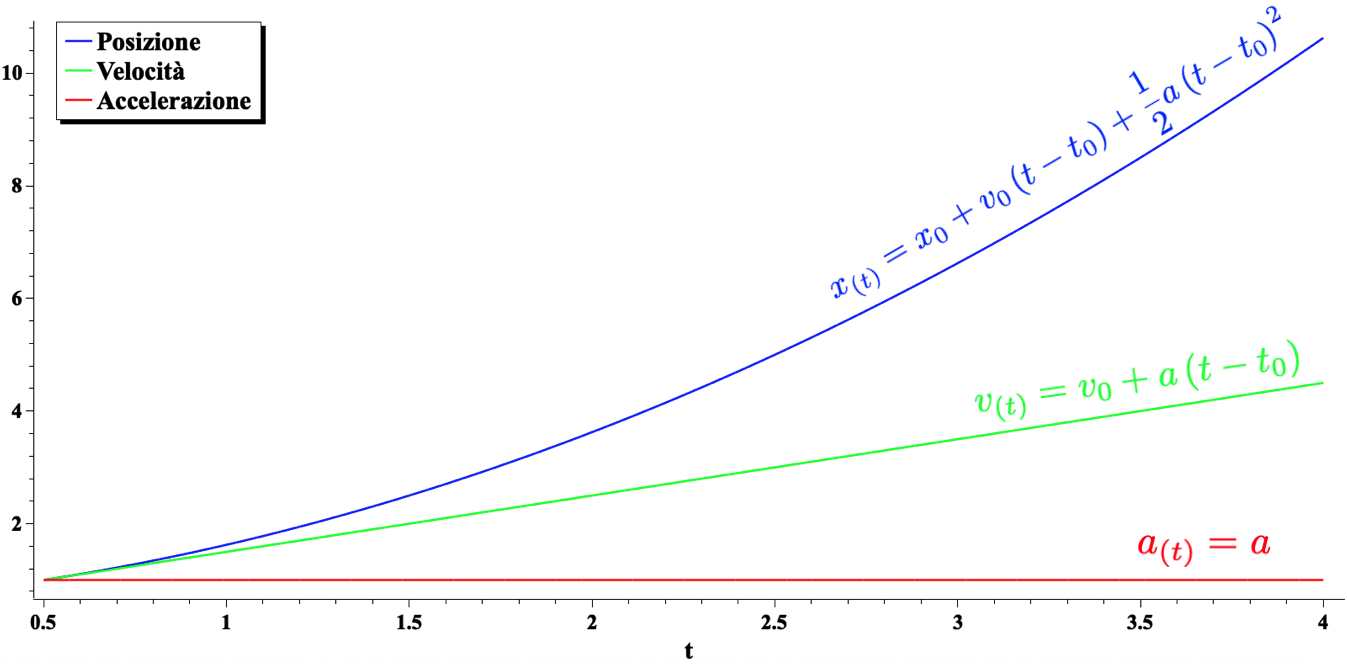
\includegraphics[width=13cm]{images/Motorettunifacc1.png} 
        \caption{Un esempio del grafico di accelerazione (rosso), velocità
        (verde) e posizione (blu), nel moto uniformemente accelerato
        unidimensionale. L'asse delle ascisse rappresenta il tempo,
        mentre quello delle ordinate la variabile dipendente.}       
    \end{center}
\label{fig:MRUA}
\end{figure}
\section{Moto armonico semplice}
%---------------------------------------------------------------------------
Il moto armonico semplice è un tipo di moto, periodico, che avviene in una
regione confinata dello spazio.\\
Prendiamo il caso in cui un punto materiale che oscilla tra una posizione minima
ed una massima, nel caso più generale possibile possiamo scrivere la sua
legge oraria utilizzando una funzione armonica.
\begin{equation}
    \boxed{x_{(t)} = A\sin\sx \omega t +\phi\dx}
\label{eq:MA}
\end{equation}
Dove $A$ è l'ampiezza di oscillazione, il punto si muove tra $ x = -A$ ed
$x = A$.\\
$\omega$ è la pulsazione, $\omega = 2\pi\nu$ dove $\nu$ è la frequenza ed
indica in numero di oscillazioni effettuate in un secondo.\\
$\phi$ è lo sfasamento iniziale, è collegato alla posizione iniziale tramite:
$ x_0 \coloneqq x_{(0)} = A\sin\phi$\\
Una volta nota la legge oraria è immediato calcolare velocità ed accelerazione,
dato che basta derivare rispetto al tempo.\\
Introduciamo ora una notazione molto utilizzata in fisica ovvero, l'utilizzo
di un punto posto sopra il simbolo di una grandezza per indicarne la
derivata totale rispetto al tempo.
\begin{equation}
    v_{(t)} = \dot x_{(t)} = A\omega\cos\sx\omega t +\phi\dx
\label{eq:MA_velocity}
\end{equation}
\begin{equation}
    a_{(t)} = \dot v_{(t)} = \ddot x_{(t)} = -A\omega^2\sin\sx\omega t +\phi\dx
\label{eq:MA_acceleration}
\end{equation}
Possiamo notare che esiste una relazione tra accelerazione e posizione.

\subsection{Equazione differenziale dell'oscillatore armonico}

Come si può notare chiaramente, l'accelerazione è direttamente proporzionale
alla posizione.
\begin{equation}
    \ddot x = -\omega^2x\seg \boxed{\ddot x_{(t)} + \omega^2x_{(t)} = 0}
\label{eq:DE_armosc}
\end{equation}
La (\ref{eq:DE_armosc}) è un'equazione differenziale al secondo ordine,
a coefficienti costanti, omogenea. Che unita alle due condizioni iniziali:\\
$x_{(0)} = A\sin\phi$ ed $\dot x_{(0)} = A\omega\cos\phi $ ha come soluzione
la (\ref{eq:MA}).\\
Ora che sappiamo che $a_{(x)} = -\omega^2x$ possiamo utilizzare la formula
(\ref{eq:v(x)_gen}) per ottenere $v_{(x)}$.
\begin{equation}
    \boxed{v^2_{(x)} = v_0^2 - \omega^2\sx x^2 - x_0^2\dx}
\label{eq:v(x)_MA}
\end{equation}

\begin{figure}[htbp]
    \begin{center}
        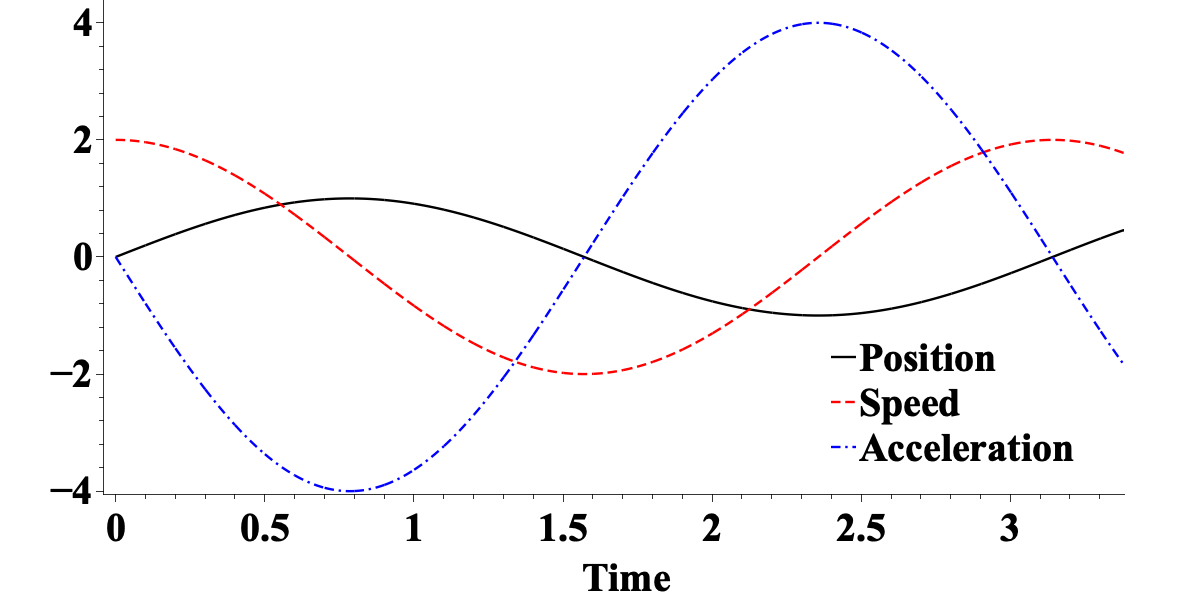
\includegraphics[width=13cm]{images/MA.png} 
        \caption{Un esempio del grafico di accelerazione (blu), velocità
        (rosso) e posizione (nero), nel moto armonico semplice.
        }
    \end{center}
\label{fig:MA}
\end{figure}
\section{Moto rettilineo smorzato esponenzialmente}
\label{section:MRSE}
%---------------------------------------------------------------------------
Questo tipo di moto si incontra quando si ha un'accelerazione proporzionale
alla velocità con coefficiente negativo (altrimenti sarebbe forzato esponenzialmente nel tempo). Introduciamo quindi un parametro di smorzamento $\beta>0$.
\begin{equation*}
    a_{(t)} = -\beta v_{(t)} = \dot v_{(t)}\seg \frac{\dot v}{v} =
    -\beta \seg \int_{t_0}^{t}dt' \frac{\dot v}{v} =  -\beta\int_{t_0}^{t}dt'\seg
\end{equation*}
\begin{equation}
    \seg\ln{\left[ \frac{v_{(t)}}{v_0}\right]} =
    -\beta\sx t-t_0\dx\seg \boxed{v_{(t)} = v_0e^{-\beta\sx t-t_0\dx}} = \dot x 
\end{equation}
\begin{equation}
    \boxed{x_{(t)} = x_0 + \frac{v_0}\beta\left[1-e^{-\beta\sx t-t_0\dx}\right]}
\label{eq:MRSE}
\end{equation}
\begin{equation}
    a = -\beta \cancel{v} = \cancel{v}\frac{dv}{dx}\seg
    \boxed{v_{(x)} = v_0 - \beta\sx x - x_0\dx}
\label{eq:v(x)_MRSE}
\end{equation}

\begin{figure}[htbp]
    \begin{center}
        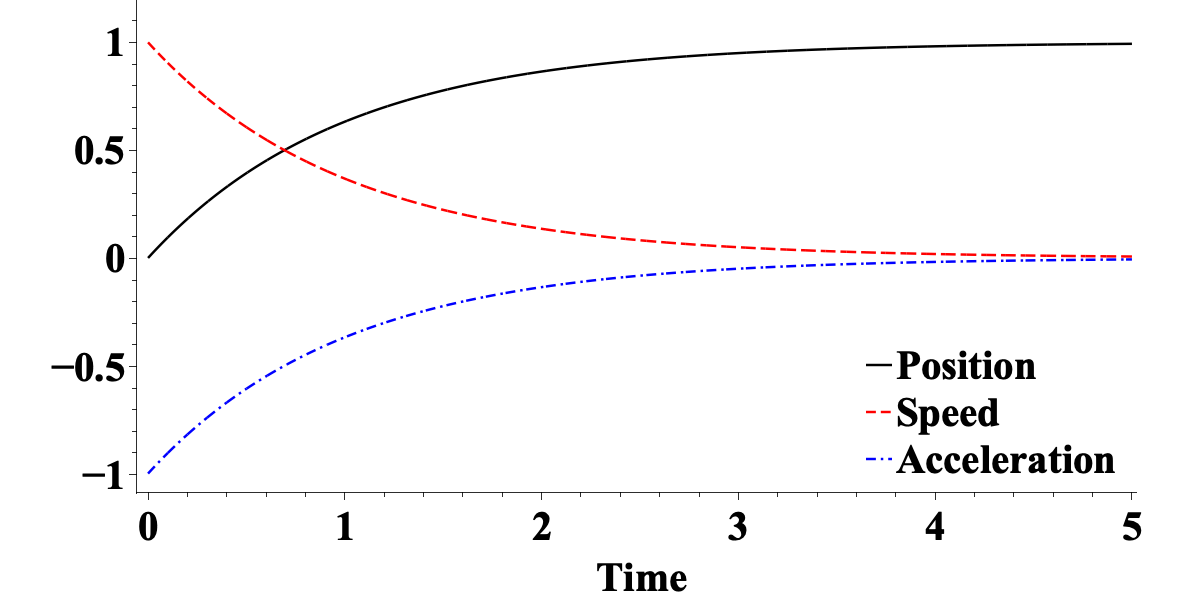
\includegraphics[width=13cm]{images/MRSE.png} 
        \caption{Un esempio del grafico di accelerazione (rosso), velocità (verde)
        e posizione (blu), nel moto smorzato esponenzialmente. L'asse delle
        ascisse rappresenta il tempo, mentre quello delle ordinate
        la variabile dipendente.}
    \end{center}
\label{fig:MRSE}
\end{figure}
\section{Coordinate curvilinee e coordinate polari nel piano}
%---------------------------------------------------------------------------
In moti casi in fisica risulta particolarmente conveniente utilizzare 
tipologie diverse di coordinate, rispetto a quelle cartesiane. Due di queste sono le coordinate curvilinee e quelle polari.\\
Le coordinate cartesiane identificano la posizione di un punto materiale 
mediante tre coordinate, corrispondenti alla proiezione del punto lungo gli assi cartesiani. Utilizzando i versori canonici $\hat\imath$, $\hat\jmath$ e $\hat k$ possiamo scrivere:
\begin{equation}
    \vec x = \sx x, y, z\dx = x\hat\imath + y\hat\jmath + z\hat k\seg
    \vec v = \dot x\hat\imath +\dot y\hat\jmath +\dot z\hat k\quad\quad
    \vec a = \ddot x\hat\imath +\ddot y\hat\jmath +\ddot z\hat k
\label{eq:Cartesian}
\end{equation}
Le coordinate curvilinee identificano come posizione, la distanza effettivamente percorsa dal punto materiale, e utilizzano come direzioni principali quella tangente $(\hat\tau)$ e quella normale $(\hat n)$.\\

\begin{figure}[htbp]
    \begin{minipage}[b]{0.47\textwidth}
        \centering
            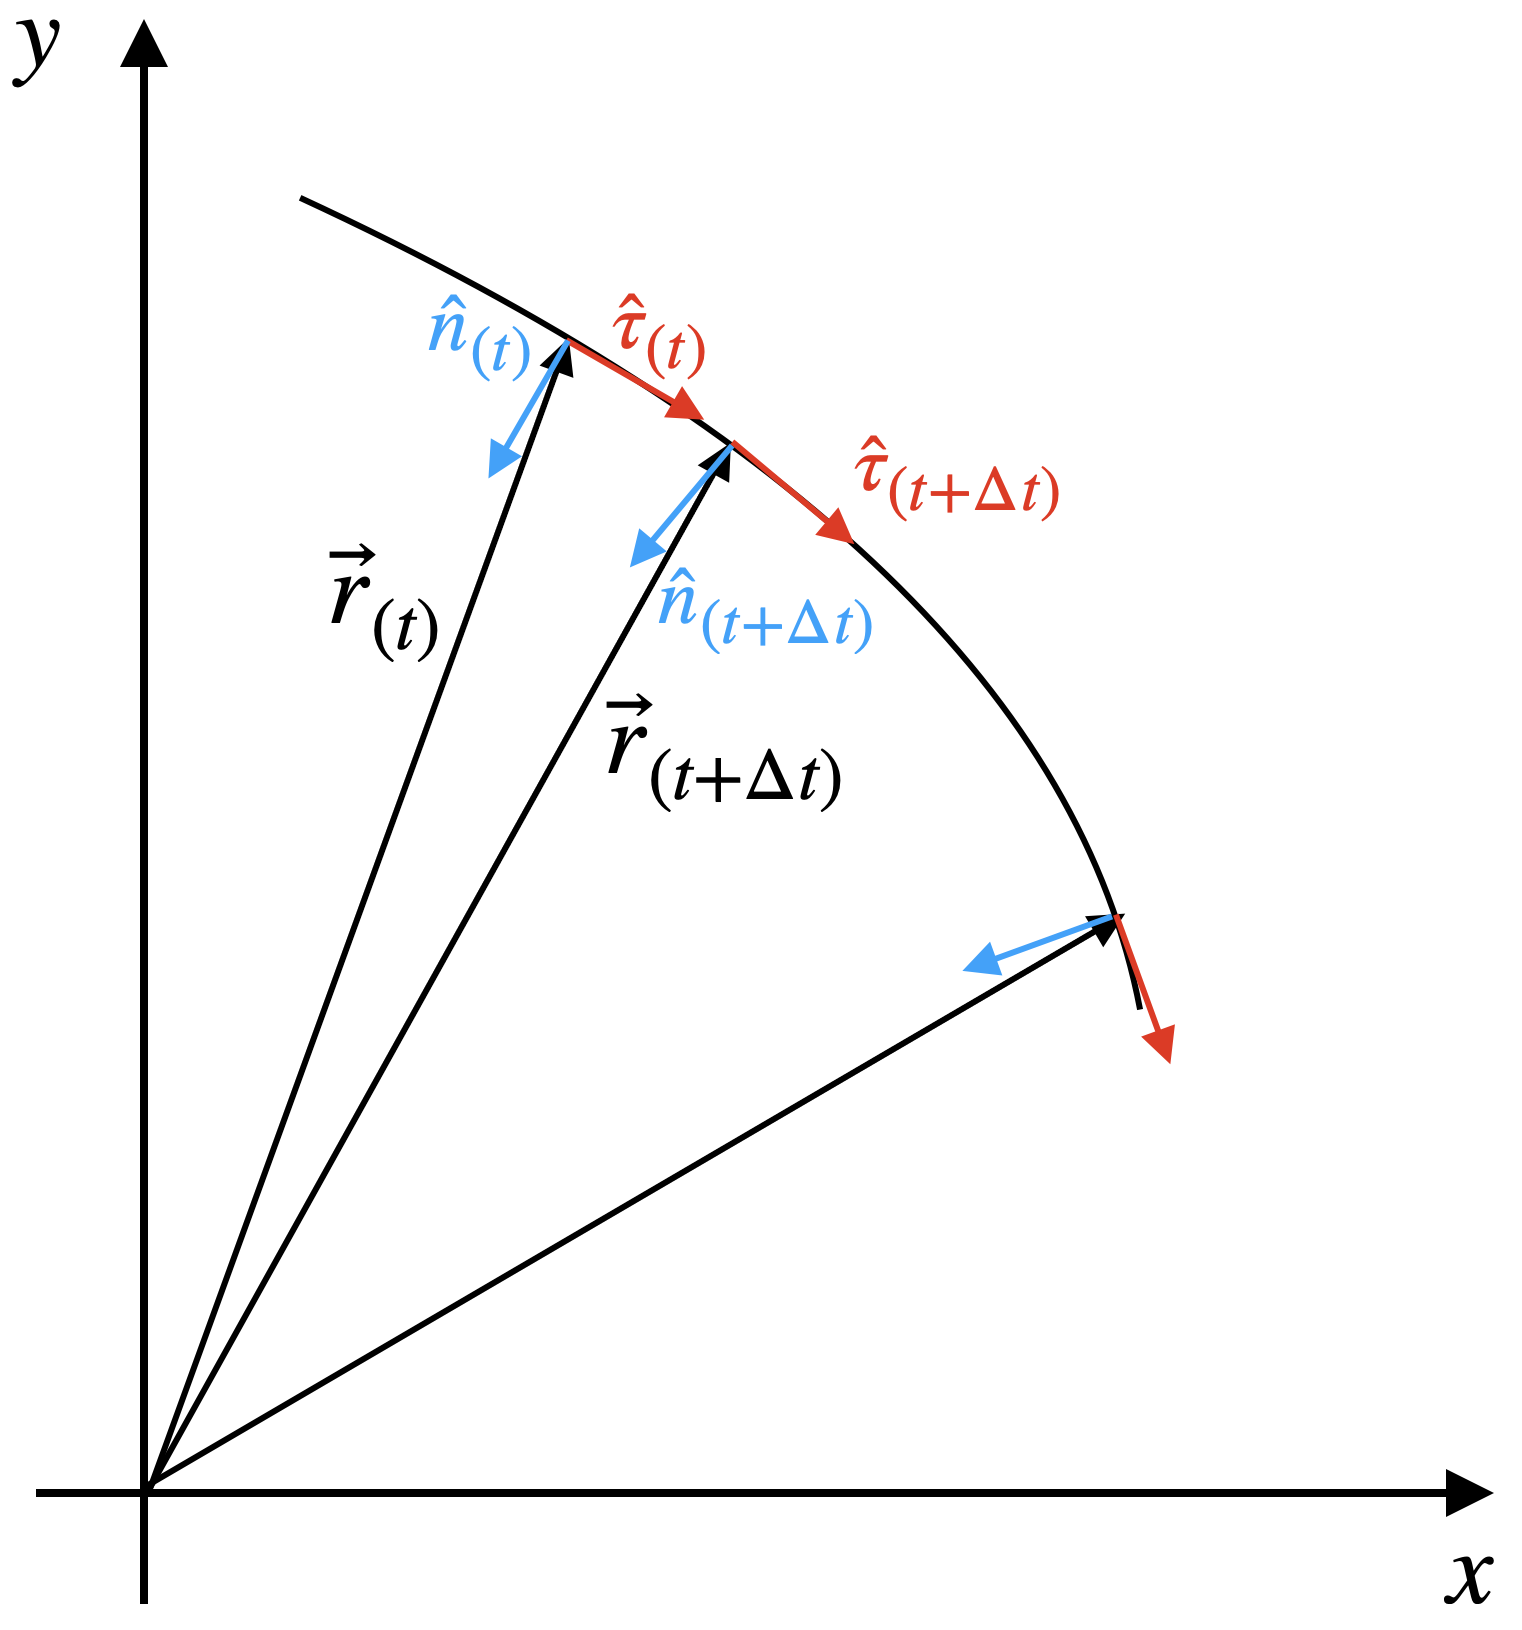
\includegraphics[width=7cm]{images/coordcurv.png}
            \caption{Rappresentazione dei versori tangente e normale lungo un tratto di curva.}
    \label{fig:curvilines}
    \end{minipage}
    \hfill
    \begin{minipage}[b]{0.47\textwidth}
        \centering
            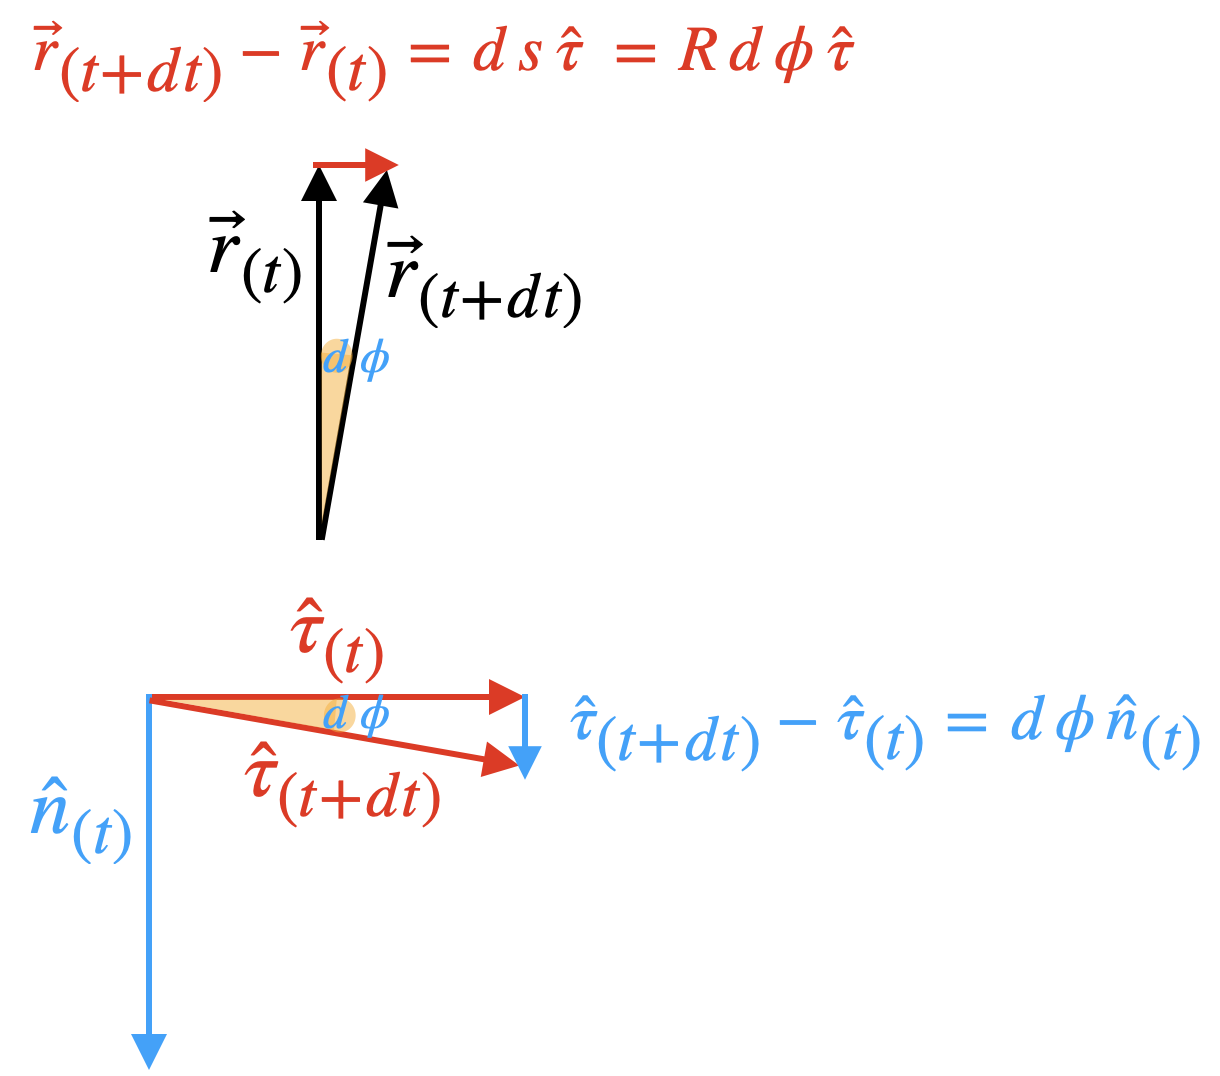
\includegraphics[width=7cm]{images/drdtau.png}
            \caption{Rappresentazione grafica della variazione infinitesima del vettore $\vec r$ e del versore $\hat\tau$.}
    \label{fig:drdtau}
    \end{minipage}
    \hfill
\end{figure}

\begin{equation}
    d\vec x = ds\hat\tau\seg \vec v = \dot s \hat\tau = v\hat\tau\seg
    \vec a = \ddot s\hat\tau + \dot s\dot\phi\hat n
\end{equation}
\begin{equation}
    \dot\phi = \frac{d\phi}{ds}\dot s = \dot s \frac{d\phi}{Rd\phi} =
    \frac{v}{R}
\label{eq:omega}
\end{equation}
\begin{equation}
    \boxed{\vec v = v\hat\tau}\quad\quad \boxed{\vec a =
    \dot v \hat\tau + \frac{v^2}{R}\hat n = a_t\hat\tau + a_n\hat n}
\label{eq:curvilines}
\end{equation}                                                                                                                                                                                                                                                                                                                                                                                                                                                                                                                                                                                                                                                                                                                                                                                                                                                                                                                                                                                                                                                                                                                                                                                                                                                                                                                                                                                                                                                                                                                                                                                                                                                                                                                                                                                                                                                                                                                                                                                                                                                                                                                                                                                                                                                                                                                                                                                                                                                                                                                                                                                                                                                                                                                                                                                                                                                                                                                                                                                                                                                                                                                                                                                                                                                                                                                                                                                                                                                                                                                                                                                                                                                                                                                                                                                                                                                                                                                                                                                                                                                                                                                                                                                                                                                                                                                                                                                                                                                                                                                                                                                                                                                                                                                                                                                                                                                                                                                                                                                                                                                                                                                                                                                                                                                                                                                                                                                                                                                                                                                                                                                                                                                                                                                                                                                                                                                                                                                                                                                                                                                                                                                                                                                                                                                                                                                                                                                                                                                                                                                                                                                                                                                                                                                             
L'accelerazione in coordinate curvilinee ha due componenti, una tangente ed una normale o centripeta. La velocità invece è sempre tangente alla traiettoria percorsa.\\
Per quanto riguarda invece le coordinate polari, si scelgono come direzioni principali quella radiale $(\hat r)$ e quella trasversa $(\hat\phi)$.

\begin{figure}[htbp]
    \centering
        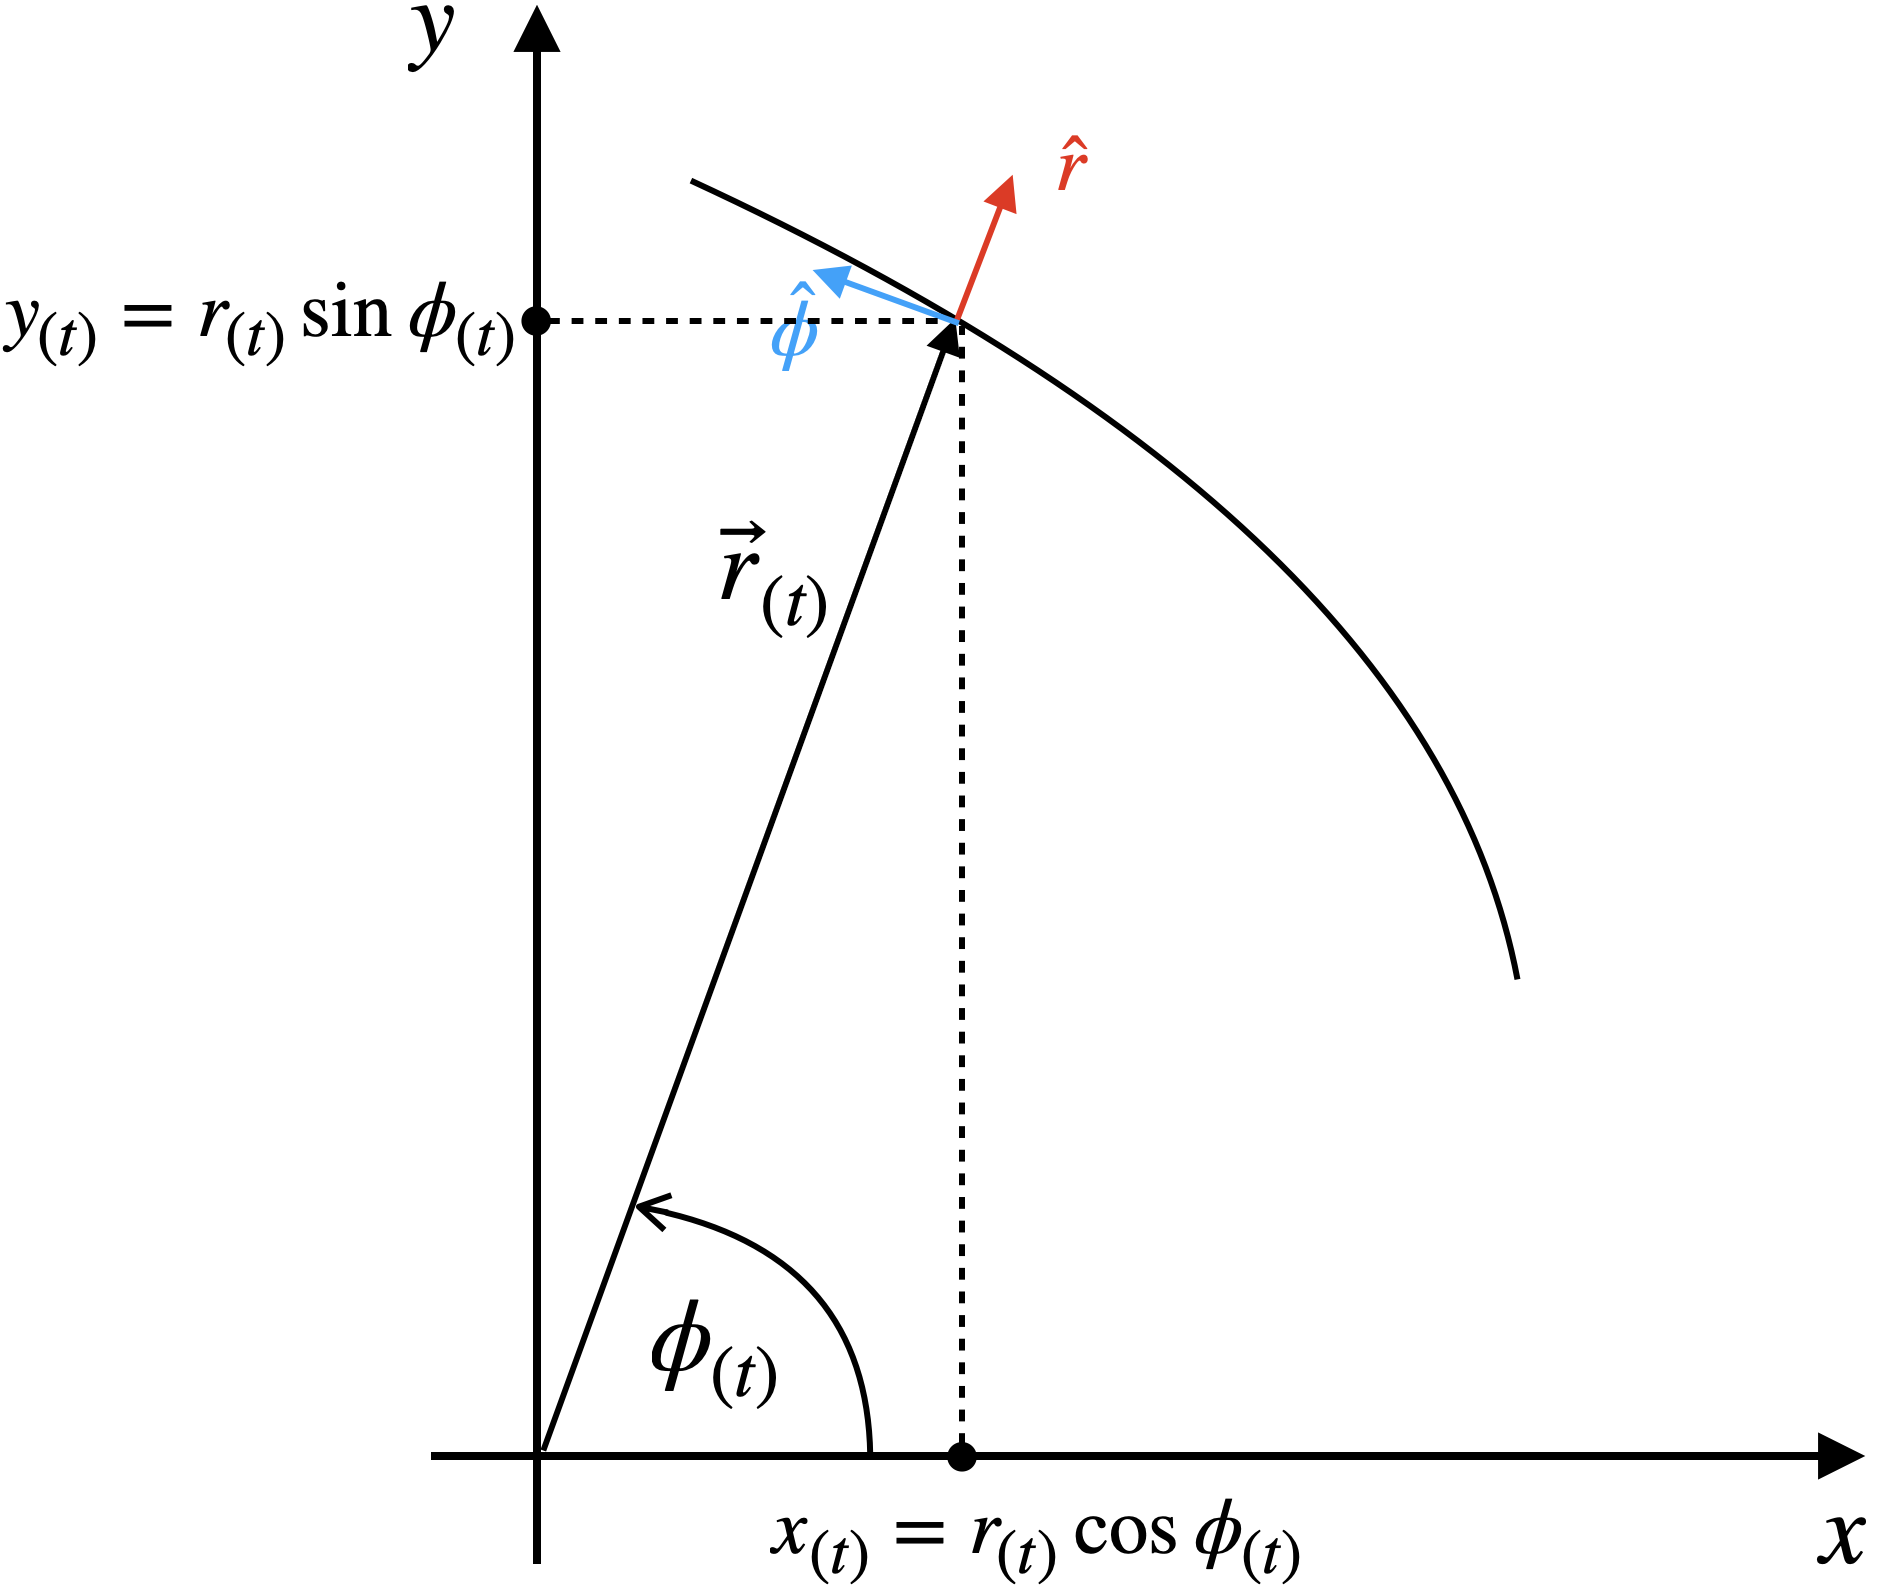
\includegraphics[width=7cm]{images/coordpol.png}
        \caption{Rappresentazione dei versori tangente e normale lungo un tratto di curva.}
\label{fig:polaris}
\end{figure}

\begin{equation}
    \boxed{\vec x = r\hat r} \seg \boxed{\vec v = \dot r \hat r +
    r\dot\phi\hat\phi}
\label{eq:polaris_xv}
\end{equation}
Per ottenere l'espressione dell'accelerazione in coordinate polari è
necessario svolgere alcuni calcoli.
\begin{equation}
    \vec a = \frac{d\vec v}{dt} = \frac{d}{dt}\sx \dot r \hat r +
    r\dot\phi\hat\phi \dx = \ddot r\hat r + \dot r\frac{d\hat r}{dt} +
    \dot r \dot \phi \hat\phi + r\ddot\phi\hat\phi + r\dot\phi\frac{d\hat \phi}{dt}
\end{equation}
\begin{equation}
    \frac{d\hat r}{dt} = \dot\phi\hat\phi\quad\quad\quad
    \frac{d\hat \phi}{dt} = -\dot\phi\hat r
\end{equation}
\begin{equation}
    \vec a = \sx \ddot r - r\dot\phi^2\dx\hat r + \sx 2\dot r\dot\phi +
    r\ddot\phi\dx\hat\phi
\end{equation}
$$\Downarrow$$
\begin{equation}
    \boxed{\vec a = \sx \ddot r - r\dot\phi^2\dx\hat r +
    \left[\frac{1}{r}\frac{d}{dt} \sx r^2\dot\phi\dx\right]\hat\phi =
    a_r\hat r + a_{\phi}\hat\phi}
\label{eq:polaris_a}
\end{equation}
\section{Moto circolare uniforme}
%-----------------------------------------------------------------------------
Un moto circolare è un moto planare in cui il punto materiale descrive come
traiettoria una circonferenza. Esso può essere scomposto in due moti armonici. Il moto circolare uniforme è chiamato in questo modo perché avviene a velocità angolare $(\omega)$ costante.
Usiamo come coordinate principali quelle curvilinee.

\begin{equation}
    s_{(t)} = R\phi_{(t)}\seg \phi = \frac sR\seg \omega = \dot \phi = \frac vR
\end{equation}
\\
Otteniamo la relazione:
\begin{equation}
    \boxed{v = \omega R}
\label{eq:v=wr}
\end{equation}
\\
Ora esattamente come abbiamo fatto nel paragrafo $(1.1)$ calcoliamo la 
legge oraria per la variabile $\phi$.

\begin{equation}
    \omega_{(t)} = \dot\phi \seg \phi_{(t)} = \phi_0 + \int_{t_0}^{t}dt'
    \omega_{(t')}\quad\quad \omega_{(t)} = \omega_0
\end{equation}
\\
\begin{equation}
    \boxed{\phi_{(t)} = \phi_0 +\omega_0\sx t - t_0\dx}
\label{eq:MCU}
\end{equation}
\\
\begin{equation}
    v = \omega_0R\seg a = a_n = \frac{v^2}R = \omega_0^2R
\label{eq:an}
\end{equation}
\\
Il periodo di rotazione è:
\begin{equation}
    T = \frac1\nu = \frac{2\pi}{\omega_0} = \frac{2\pi R}v
\label{eq:period}
\end{equation}
\section{Moto circolare uniformemente accelerato}
%-----------------------------------------------------------------------------
Il moto circolare non uniforme si ha quando la velocità angolare non è
costante nel tempo. Questo comporta che la componente tangente di $\vec a$ non è nulla. Nel caso in cui $\omega$ è lineare nel tempo si avrà un moto circolare uniformemente accelerato.
\\ Definiamo quindi l'accelerazione angolare:
\begin{equation}
    \alpha_{(t)} = \dot \omega = \ddot \phi\seg a_t = \dot v =
    \frac d{dt}\sx \omega R\dx = \alpha R
\end{equation}
Di conseguenza avremo che:
\begin{multline}
    \omega_{(t)} = \omega_0 + \int_{t_0}^tdt'\alpha_{(t')}  = \omega_0 + \alpha_0\sx t - t_0\dx \seg
    \\\boxed{\phi_{(t)} = \phi_0 + \omega_0\sx t - t_0\dx+ \frac12\alpha_0\sx t - t_0\dx^2}
\end{multline}
Esiste anche un analogo della formula (\ref{eq:v(x)_0}).
\begin{equation}
    \alpha =\dot \omega = \frac{d\omega}{d\phi}\dot\phi\seg
    \boxed{\omega^2_{(\phi)} = \omega_0^2 + 2\alpha_0\sx\phi-\phi_0\dx}
\label{eq:w(phi)}
\end{equation}
Osservando la figura (\ref{fig:rotantvector}), possiamo scrivere la relazione
tra velocità e velocità angolare con un formalismo verroriale:

\begin{figure}[htbp]
    \centering
        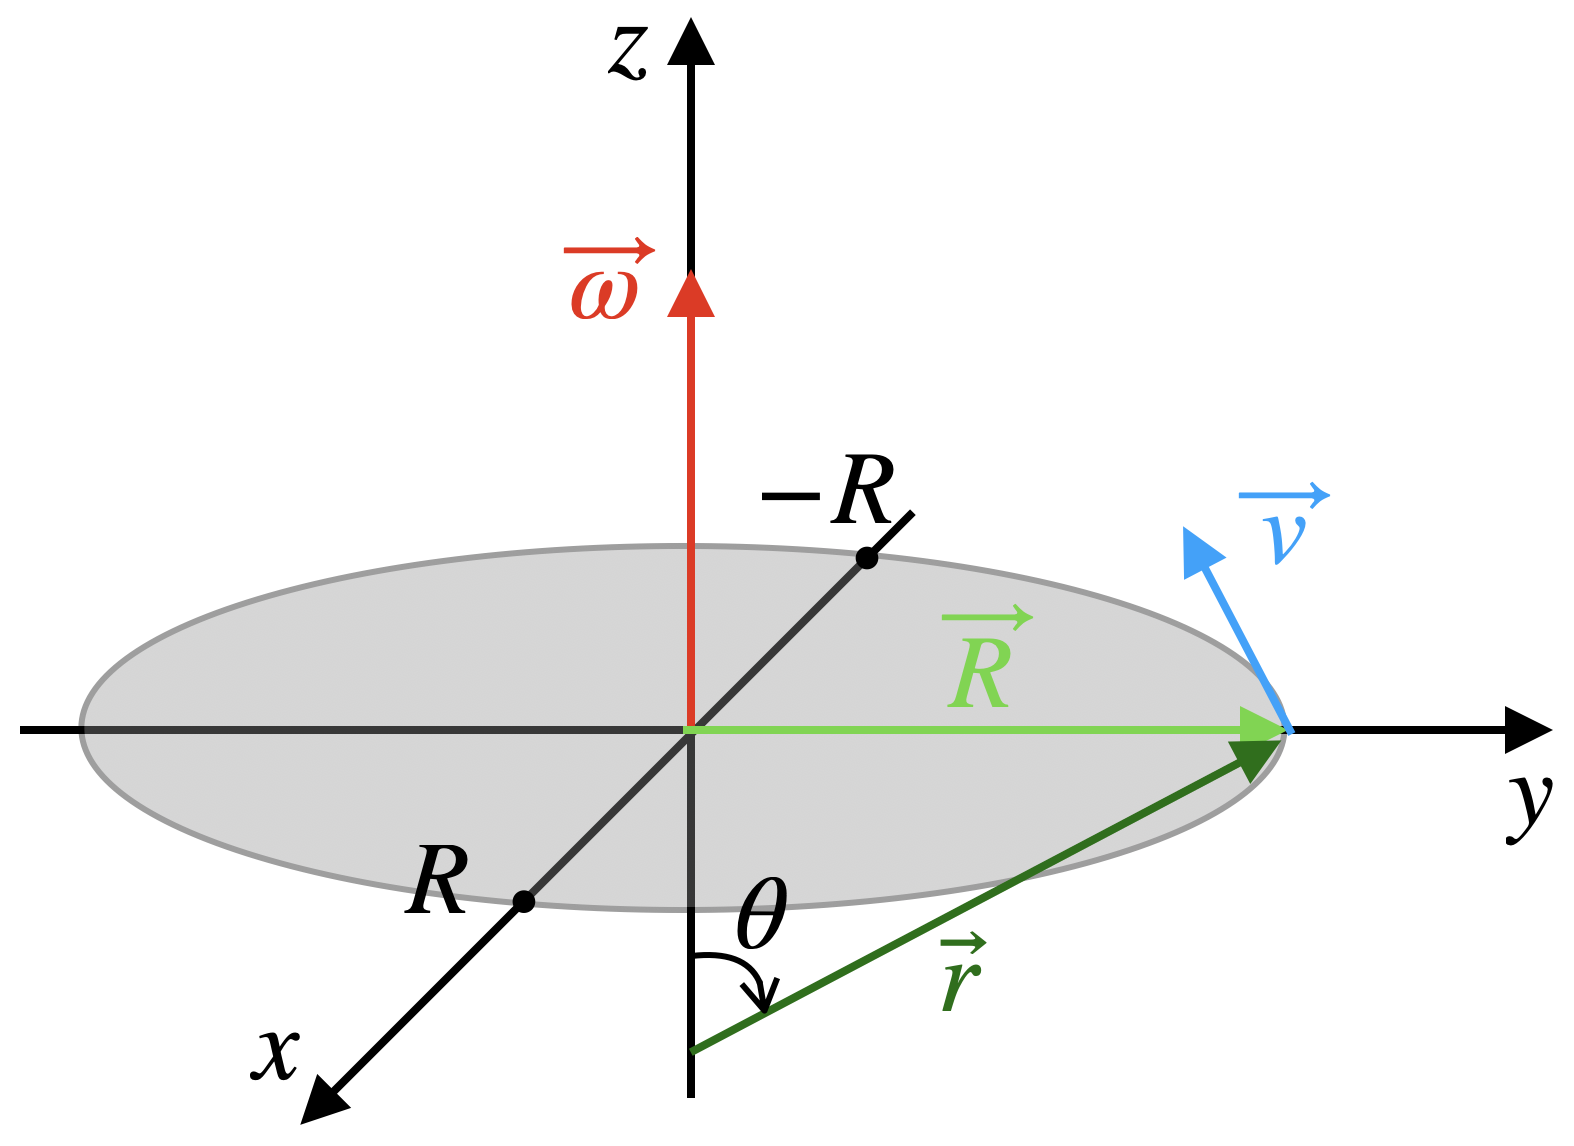
\includegraphics[width=7cm]{images/ovetr.png}
        \caption{Rappresentazione dei vettori $\vec\omega$ e $\vec v$ in un moto
        circolare per $\vec R$ e di precessione per $\vec r$.}
\label{fig:rotantvector}
\end{figure}

\begin{equation}
    \vec v = \vec\omega\times\vec R\seg \left| \vec v \right|  = \omega R
\end{equation}
Se trasliamo verso il basso l'origine degli assi otteniamo che:
\begin{equation}
    \vec v = \vec\omega\times\vec r\seg \left| \vec v \right|  = \omega r\sin\theta = \omega R
\label{eq:v(w)}
\end{equation}
Ne segue che dato un vettore generico rotante $\vec A$ avremo che:
\begin{equation}
    \frac{d\vec A}{dt} = \vec\omega\times\vec A
\label{eq:rotantvector}
\end{equation}
Infine scriviamo la forma dell'accelerazione.
\begin{equation}
    \vec a = \frac d{dt}\sx\vec\omega\times\vec r\dx =
    \vec \alpha\times \vec r + \vec\omega\times\vec v
\label{eq:a_vec}
\end{equation}
Come possiamo notare se consideriamo il caso particolare in cui $\alpha = 0$
otteniamo:
\begin{equation}
    \vec a = \vec \omega\times\vec v = \vec \omega\times\sx \vec\omega\times
    \vec R\dx = \cancel{\sx\vec\omega\cdot\vec R\dx}\vec\omega - \omega^2\vec R
    = \omega^2R\hat n = \frac{v^2}R\hat n
\label{eq:an_vec}
\end{equation}
Possiamo decomporre il moto circolare in due moti armonici, uno per l'asse $x$ ed uno per l'asse $y$.
\begin{equation}
    \begin{cases}
        x_{(t)} = R\cos\phi_{(t)}\\
        y_{(t)} = R\sin\phi_{(t)}\\
    \end{cases}\seg
    \begin{cases}
        \dot x_{(t)} = -R\dot\phi\sin\phi_{(t)}\\
        \dot y_{(t)} = R\dot\phi\cos\phi_{(t)}
    \end{cases}
\label{eq:components}
\end{equation}

\begin{figure}[htbp]
    \centering
        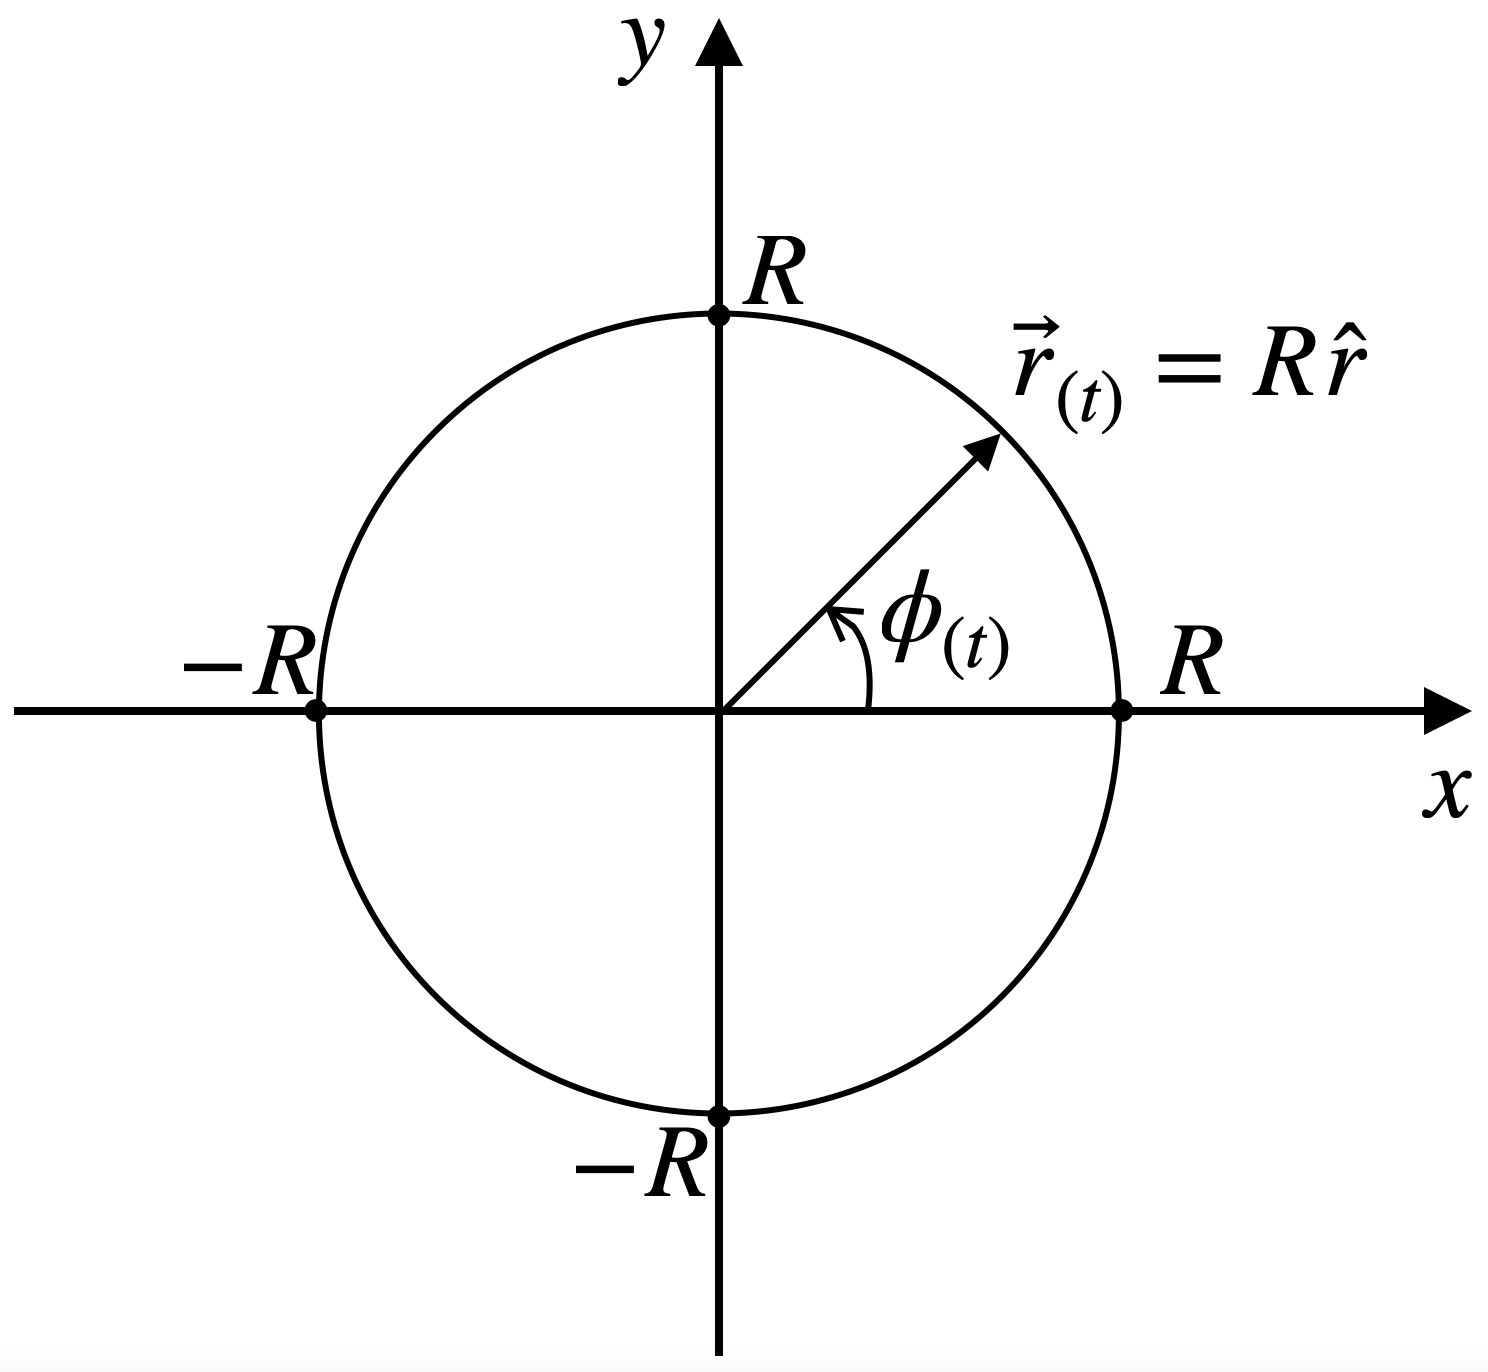
\includegraphics[width=7cm]{images/circ.png}
        \caption{Rappresentazione della traiettoria, del raggio vettore e della variabile angolare $\phi$ nel moto circolare.}
\label{fig:circ}
\end{figure}
\section{Moto parabolico}
%-----------------------------------------------------------------------------
Un moto parabolico è il moto che compie un proiettile lanciato con una
certa velocità $\vec v_0$, sottoposto ad un campo di forze uniforme e
costante, ovvero il campo gravitazionale in prossimità della superficie
terrestre.\\
Il moto parabolico può essere scomposto in due moti disaccoppiati,
un moto rettilineo uniforme lungo l'asse $x$ ed un moto rettilineo
uniformemente accelerato lungo l'asse $y$. Questo perché non sono presenti
forze orizzontali, e l'unica forza agente sul corpo è quella gravitazionale
in direzione verticale. Dunque è presente un'accelerazione pari a:
$\vec a = -g\hat\jmath $. Per semplicità poniamo l'istante iniziale $ t_0 = 0$.

\begin{equation}
    \begin{cases}
        x_{(t)} = x_0 + v_0\cos\phi t\\
        y_{(t)} = y_0 + v_0\sin\phi t - \frac12 g t^2
    \end{cases}\seg
    \begin{cases}
        \dot x_{(t)} = v_0\cos\phi \\
        \dot y_{(t)} = v_0\sin\phi - gt
    \end{cases}
\label{eq:MP}
\end{equation}
\\
Si può anche ricavare l'equazione della traiettoria, isolando il tempo
dalla legge oraria per $x$ ed inserendolo nell'equazione per $y$.

\begin{equation}
    t = \frac{x-x_0}{v_0\cos\phi}\seg y_{(x)} =
    y_0 + \tan\phi\sx x-x_0\dx-\frac{g}{2v_0^2\cos^2\phi}\sx x-x_0\dx^2
\label{eq:MP_y(x)}
\end{equation}
\\
Come si può notare è l'equazione di una parabola centrata in $x_0$ con
coefficiente del termine di secondo grado sempre negativo, stante ad
indicare che la traiettoria parabolica ha sempre la concavità rivolta
verso il basso, come è giusto che sia dato che il punto materiale dovrà
cadere a terra.
\\ Imponendo la $y$ uguale a zero, possiamo ricavare il tempo di volo.

\begin{equation}
    y_0 + v_0\sin\phi \tau - \frac12 g \tau^2 = 0 \seg
    \boxed{\tau = \frac{v_0}{g}\sin\phi + \sqrt{\frac{v_0^2}{g^2}\sin^2\phi+2\frac{y_0}g}}
\label{eq:flytime}
\end{equation}
\\
Calcolando $x_{(\tau)}$ oppure imponendo uguale a zero $y_{(x)}$, otterremo
la gittata del proiettile, ovvero la massima distanza percorsa lungo
l'asse orizzontale.

\begin{equation}
    \boxed{R = x_0 + \frac{v_0^2}{g}\sin\sx\phi\dx\cos\sx\phi\dx +
    v_0\cos\phi\sqrt{\frac{v_0^2}{g^2}\sin^2\phi+2\frac{y_0}g}}
\label{eq:range}
\end{equation}
\\
Se consideriamo il caso in cui il proiettile parte da terra,
abbiamo che $y_0 = 0$ quindi la gittata diventerà:

\begin{equation}
    R = x_0 +2\frac{v_0^2}{g}\sin\sx\phi\dx\cos\sx\phi\dx = x_0 + \frac{v_0^2}{g}\sin\sx2\phi\dx
\label{eq:range_0}
\end{equation}
\\
Il valore massimo di questa $R$ si ottiene quando il $\sin\sx2\phi\dx$ è
pari ad 1, dunque la gittata massima si otterrà per $\phi = 45^\circ$.
Dobbiamo ricordare che nel caso in cui $x_0\ne0$, $R$ rappresenta
ovviamente l'ascissa del punto in cui il proiettile cade a terra.
Quindi per calcolare la distanza effettivamente percorsa, si deve
considerare la differenza $R-x_0$.
Per quanto riguarda invece la quota massima raggiunta dal proiettile,
bisogna annullare la $\dot y_{(t)}$ per ricavare il tempo in cui si
raggiunge tale quota (velocità verticale nulla).

\begin{equation}
    t^* = \frac{v_0}{g}\sin\phi\seg\boxed{h = y_0 + \frac{v_0^2}{2g}\sin^2\phi}
\label{eq:h_max}
\end{equation}
\\
\begin{figure}[h]
        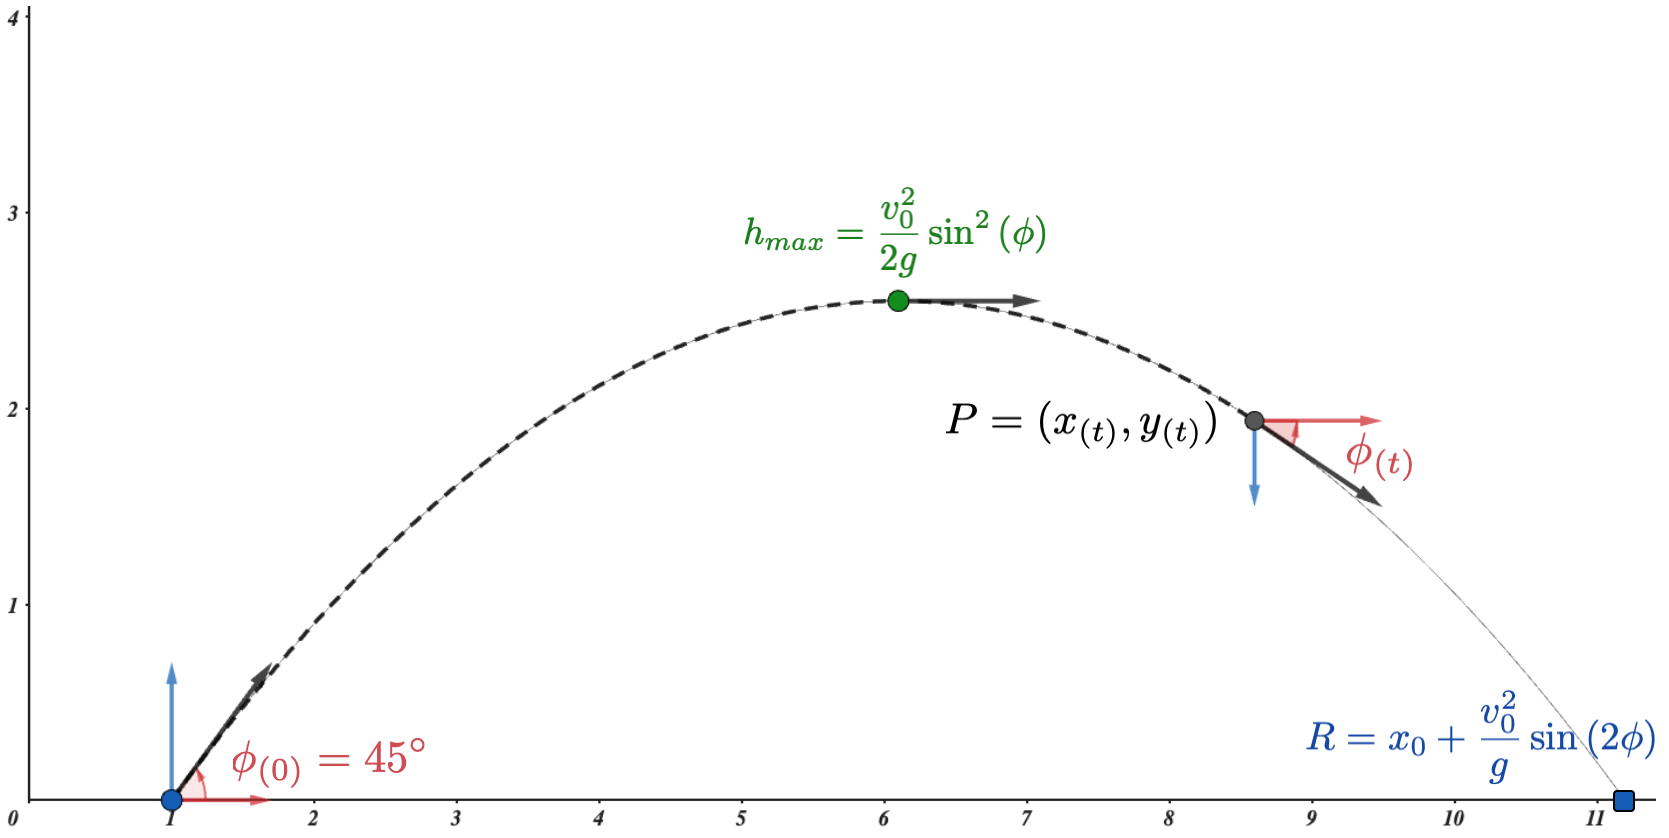
\includegraphics[width=0.9\textwidth]{images/MP1.png} 
        \caption{Esempio di una traiettoria di un moto parabolico con $\phi = 45^\circ$.
        Sono stati riportati Il punto iniziale in blu, il punto a quota
        massima in verde, un punto generico in nero ed il punto ad ascissa
        massima.}
\label{fig:MP}
\end{figure}
Se consideriamo la distanza orizzontale percorsa \emph{(gittata o range)}, oltre
al fatto di presentare un massimo $\phi = 45^\circ$, possiamo notare che si avranno
gittate uguali per angoli di lancio complementari.\\
Mostriamo qualche esempio nelle figure (\ref{fig:MP}) e (\ref{fig:MP_2}).

\begin{figure}[h]
        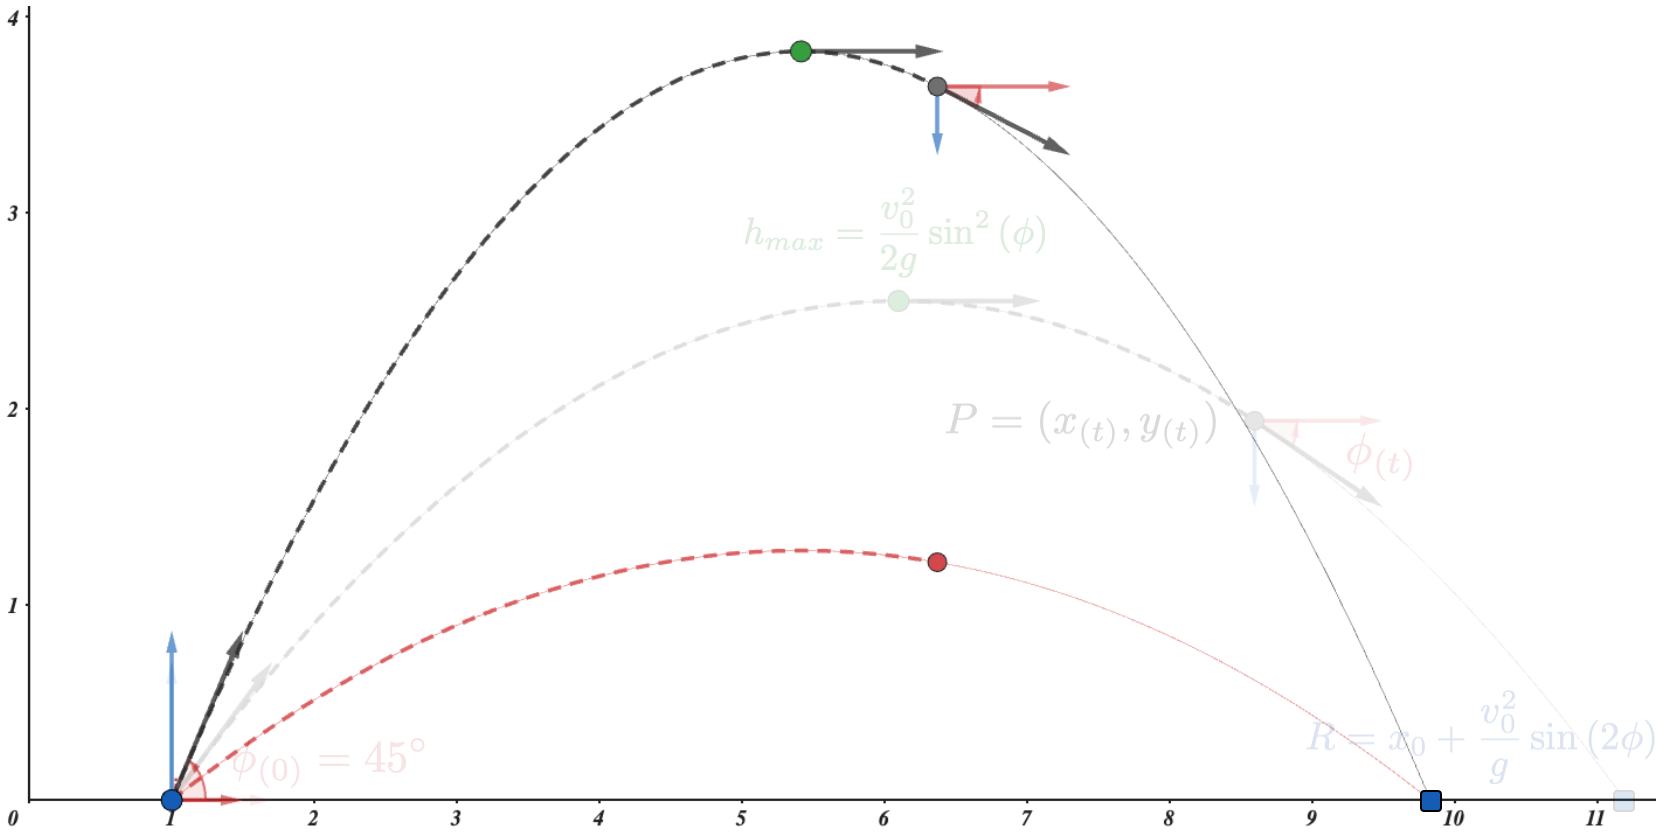
\includegraphics[width=0.9\textwidth]{images/MP2.png} 
        \caption{Rappresentazione di due traiettorie con stessa gittata.
        $\phi = 30^\circ$ in rosso e $\phi = 60^\circ$ in nero.}
\label{fig:MP_2}
\end{figure}